% Set options for wide aspect ratio and beamer document class
\documentclass[aspectratio=169]{beamer}

% Package imports
\usepackage{fontspec}
\usepackage{epigraph}
\usepackage{xcolor}
\usepackage[percent]{overpic}

%for speaker notes.
\usepackage{pgfpages}
\setbeameroption{show notes on second screen}

% custom options to make epigraph look good on a beamer slide
\renewcommand{\epigraphrule}{0pt}
\setlength{\epigraphwidth}{.9\textwidth}
\renewcommand{\textflush}{flushepinormal}

\newcommand\blfootnote[1]{%
  \begingroup
  \renewcommand\thefootnote{}\footnote{#1}%
  \addtocounter{footnote}{-1}%
  \endgroup
}

% default document font specifications
\setmainfont{FiraSans-Book}
\setsansfont{FiraSans-Book}
\definecolor{textcolour}{rgb}{255,255,255}

% Definign the Mozilla colour palette for presentations 
\definecolor{moz_dark_green}{RGB}{77,78,83}
\definecolor{moz_light_green}{RGB}{208,211,212}
\definecolor{moz_light_blue}{RGB}{0,150,221}
\definecolor{moz_dark_blue}{RGB}{0,33,71}
\definecolor{moz_accent_green}{RGB}{111,190,74}
\definecolor{moz_accent_yellow}{RGB}{255,203,0}
\definecolor{moz_accent_orange}{RGB}{255,149,0}
\definecolor{moz_accent_orange2}{RGB}{230,96,0}
\definecolor{moz_accent_red}{RGB}{193,56,50}

% new counter for column enumerates
\newcounter{savedenum}
\newcommand*{\saveenum}{\setcounter{savedenum}{\theenumi}}
\newcommand*{\resume}{\setcounter{enumi}{\thesavedenum}}

% Background for all slides set here
\setbeamertemplate{background canvas}{
\includegraphics [width=\paperwidth]{bg_alt_small.png}}

\setbeamercolor{structure}{fg=textcolour}

\setbeamerfont{title}{size = \Huge}
\setbeamercolor{normal text}{fg=textcolour}

%define specific fint size interpretations for the beamer presentation mode.
\renewcommand{\tiny}{\fontsize{7pt}{8pt}\selectfont}
\renewcommand{\scriptsize}{\fontsize{9pt}{12pt}\selectfont}
\renewcommand{\footnotesize}{\fontsize{10pt}{12pt}\selectfont}
\renewcommand{\small}{\fontsize{12pt}{18pt}\selectfont}
\renewcommand{\normalsize}{\fontsize{14pt}{18pt}\selectfont}
\renewcommand{\large}{\fontsize{16pt}{24pt}\selectfont}
\renewcommand{\Large}{\fontsize{24pt}{37pt}\selectfont}
\renewcommand{\LARGE}{\fontsize{31pt}{42pt}\selectfont}
\renewcommand{\huge}{\fontsize{48pt}{54pt}\selectfont}
\renewcommand{\Huge}{\fontsize{80pt}{96pt}\selectfont}

% remove navigation symbols
\setbeamertemplate{navigation symbols}{}
 
% After building the PDF you may ensure that local system fonts are embedded in the final PDF using:
% gs -dNOPAUSE -dBATCH -sDEVICE=pdfwrite -dPDFSETTINGS=/prepress -dEmbedAllFonts=true -sOutputFile=DN2018-lopatka-portable.pdf -f DN2018-Lopatka.pdf
% This will also compress the final output size 

\begin{document}

\begin{frame}
\frametitle{The Morphology of the Web is Changing!}
%
\begin{overpic}[width=0.7\textwidth]{morphs.png}
\put(85, 7){\large{Martin Lopatka}}
\put(78, 1){\small{mlopatka@mozilla.com}}
\put(57.25, -5){\small{Data Scientist/Applied Statistician}}
\end{overpic}
%
\end{frame}
\note[itemize]{
\item Research Engineering and Data Science at Mozilla! 
\item The world’s largest shared public resource... The Web.
\item you may have heard of it.. it's called Firefox. 
\item "the study of form and structure without consideration of function"
\item carrying out research on the nature, structure, and technology on the Modern web!
}

\begin{frame}
\frametitle{Disclaimer}
%
Martin Lopatka provides this contribution to the Data Natives 2018 conference in a personal capacity. The views expressed are his own and do not necessarily represent the views of Mozilla Corporation or the Mozilla Foundation.
% FAST!!! don't waste time here!
\end{frame}
\note{
Disclaimer! GO fast!
}

{
% alternate background slide templalte. clobbers background options with full-slide image
\usebackgroundtemplate{
\includegraphics[width=\paperwidth]{bg_alt_small-rlogo.png}}%
\begin{frame}
\begin{overpic}[width=0.7\textwidth]{2003-web-small.png}
\put(-05,90){\textbf{THE INTERNET 2003}}
\put(-05,86){\tiny{Barrett Lyon / The Opte Project}}
\end{overpic}
\end{frame}
}
\note[itemize]{
\item Paint a picture of the web’s morphology in 2003
\item Wikipedia young < 100K articles vs 6 million
\item Reddit did not exist yet, Google had just released Page-rank (household name). 
\item Facebook won’t launch until next year.
\item Op-tee project visualisation made by a massive crawl fo the web, 
\item 30 million TLDs registered.
\item links -> content creators. outbound links to other content. less log in. No SEO.
}

{
\usebackgroundtemplate{
\includegraphics[width=\paperwidth]{bg_alt_small-rlogo.png}}%
\begin{frame}
\begin{overpic}[width=0.8\textwidth]{2015-web-large-2.png}
\put(-04.5,69.5){\textbf{THE INTERNET 2015}}
\put(-04.5,66){\tiny{Barrett Lyon / The Opte Project}}
\end{overpic}
\end{frame}
}
\note[itemize]{
\item Emphasise differences in Morphology
\item Web includes over 314 Million (geo diversity)
\item more links generated algorithmically (2016 G will punish this)
\item online advertising market 125 billion dollars.
\item emergence of more hyperlinked nodes

}

\begin{frame}
\frametitle{The centrality of advertisers}
%
\large{Are trackers the new backbone of the Web?}
\footnotesize{https://medium.com/firefox-context-graph/are-trackers-the-new-backbone-of-the-web-fb800435da15}
\begin{center}
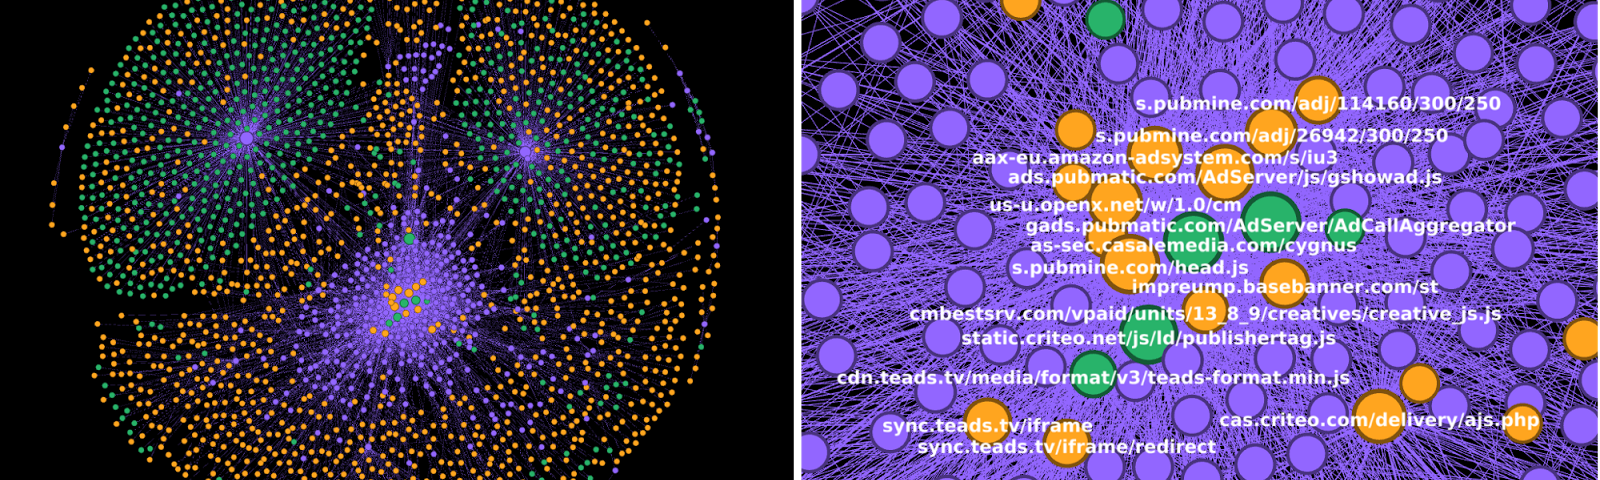
\includegraphics[width=0.85\paperwidth]{0thN-8lZ4H2_xjbkt.png}
\end{center}
%
\end{frame}
\note[itemize]{
\item investigation of these hyperlinked nodes to explore their nature 
\item we begin exploring the role of highly connected, hub nodes
\item resources accessed in a third-party context. Community detection was performed using Louvain Modularity
\item fewer hyperlinks between pages belonging to separate tracking/advertising communities
\item This is the first indication of a advertisement network influence. 
\item infrastructure: big assumptions related to actual traffic 
}

{
\usebackgroundtemplate{
\includegraphics[width=\paperwidth]{bg_alt_small-rlogo.png}}%
\begin{frame}
\frametitle{How did we get to an ecosystem of silos?}
%
\begin{itemize}
\item{40\% of total Web browsing page views can be attributed to only 65 top level domains (TLD)}
\item{Five (TLD+1) sites (Google, Facebook, Amazon, Yahoo, and Reddit) make up 22\% of all traffic
\footnote{https://medium.com/firefox-context-graph/are-trackers-the-new-backbone-of-the-web-fb800435da15}}
\item{Of the 22,310,889 domains processed, 52.63\% (11,742,112) were found to serve advertisements
\footnote{https://commecica.com/2018/06/27/web-ad-prevalence/}}
\end{itemize}
%
\end{frame}
}
\note[itemize]{
\item We’ve already made some scary discoveries about the diversity
\item "Comme ci comme ca" using the May 2018 batch of common crawl
\item Easylist ruleset ->f Adblock adblocker 
\item Morphology is changing, important to discuss traffic and therefore content access
}

\begin{frame}
%
\epigraph{Social platforms were designed to facilitate; they became attention brokers, they are designed to help companies reach users as these sort of middlemen where they know a ton about you and thats the service they are providing to the advertisers.}{Renee DiResta ``The Internet's Original Sin'' \\ 27-Oct-2018 12:45}
%
\end{frame}
\note[itemize]{
\item Mozfest, Renee DiResta: abuses of social media platforms 
\item platform purpose built for advertisement.
\item *infrastructure for advertisement* content and social platforms have evolved to "maximise sustained engagement on site"
\item Example: you consume your news, *on* facebook (60\% US)
}

{
\usebackgroundtemplate{
\includegraphics[width=\paperwidth]{bg_alt_small-rlogo.png}}%
\begin{frame}
%
The highest trafficked pages on the Web\footnote{https://www.alexa.com/topsites; accessed 20-Nov-2018 11:17} are search engines, Social media platforms, and Commerce platforms
\begin{center}
\begin{columns}[T]
  \begin{column}{.3\linewidth}
  \begin{enumerate}
	\item{Google.com}
	\item{Youtube.com}
	\item{Facebook.com}
	\item{Baidu.com}
	\item{Wikipedia.org $\star$}
    \saveenum
  \end{enumerate}
  \end{column}
  \begin{column}{.3\linewidth}
  \begin{enumerate}
    \resume
         \item{Qq.com}
	\item{Taobao.com}
	\item{Yahoo.com}
	\item{Tmall.com}
	\item{Amazon.com}  
	\end{enumerate}
  \end{column}
\end{columns}
\end{center}
%
\end{frame}
}
\note[itemize]{
\item highest trafficked pages on the web -> business model where engaged time on site is directly beneficial in a a business sense.
\item Web commerce platforms, advertisers, search engines, and Social media platforms. 
}

\begin{frame}
\frametitle{The new ecology of outbound links}
Dynamic pages feature changing content, showing different text, images and videos depending on who's visiting and when. This dynamic content includes different hyperlinks.\\\vspace{0.5cm}
%
\begin{itemize}
\item{retargeting}
\item{advertisement}
\item{realtime bidding}
\item{social linking}
\end{itemize}
%
\end{frame}
\note[itemize]{
\item Retargeting, advertiser to tag you (with a cookie) and redirect as a specific media clicker, this requires a link through an advertiser's intermediate page
\item  Advertisement content, usually dynamically generated for the individual or profile of the page visitor
\item Real Time bidding, the links surfaced may vary from one page visitor to another, based on estimates of *your* profile and value to advertisers, meaning crawlers will be served a fundamentally different page
\item Social linking, more roads lead back to the social network ecosystem.
}

\begin{frame}
%
\epigraph{The problem is that the web is no longer built upon the simple premise of a collection of small static HTML and image files served up with a simple tag structure and readily parsed with a few lines of code. Today’s web is richly dynamic, multimedia and increasingly broken into walled gardens and device-specific parallel webs.}{Kalev Leetaru ``Are Web Archives Failing The Modern Web: Video, Social Media, Dynamic Pages and The Mobile We''\\ 24-Feb-2017 22:41}
%
\end{frame}
\note[itemize]{
\item from Kalev Letaru in a 2017 Forbes article discussing the role of the internet archive and common crawl initiatives in helping us make sense of the Web!
}

{
\usebackgroundtemplate{
\includegraphics[width=\paperwidth]{bg_suit.png}}%
\begin{frame}
%
\vspace{-1cm}\hspace{-0.5cm}\begin{overpic}[height=0.8\textheight]{flow.png}
\put(85, 63.5){\large{\textbf{research and development}}}
\end{overpic}
%
\end{frame}
}
\note[itemize]{
\item leverage crawler technology for it’s robust technical measurement features. 
\item also want to user traffic patterns to ensure our feature development is relevant
\item Crawlers, have a  limited View - the open web makes up less and less of the Web.
\item  how do we study the nature of the web as people actually experience it in a Privacy respectful way that also takes advantage of scalable technology like Web crawlers?
}

\begin{frame}
\frametitle{Make Firefox better with pioneer}
%

\includegraphics[width=0.4\textwidth]{Pioneer.png}

\small{https://medium.com/firefox-context-graph/make-firefox-better-with-pioneer-10c82d0f9301}
%
\end{frame}
\note[itemize]{
\item We ask permission,
\item compliment the shortcomings of various data collection strategies
\item The Firefox Pioneer program is an opt-in data collection 
\item real human readable consent policy
}

{
\usebackgroundtemplate{
\includegraphics[width=\paperwidth]{bg_last.png}}%
\begin{frame}
\vfill
\LARGE{https://github.com/mozilla/}\\
\LARGE{overscripted/}
\end{frame}
}
\note[itemize]{
\item selective Javascript execution stack for tracking related activity 
\item 70Gb and touches over 2 million web pages seeded from the Alexa top 10K
\item aspiring or established data scientist, come get your hands dirty
\item data science can also work in a collaborative open source manner
}

\begin{frame}
\frametitle{Acknowledgements}
\begin{center}
\begin{columns}[T]
  \begin{column}{.3\linewidth}
  \begin{itemize}
	\item{Sarah Bird}
	\item{Victor Ng}
	\item{David Zeber}
	\item{Fredrik W\'ollsen}
	\item{Jason Thomas}
	\item{Steven Englehardt}
  \end{itemize}
  \end{column}
\begin{column}{.3\linewidth}
  \begin{itemize}
         \item{Ruizhi You}
	\item{Louis Belleville}
	\item{Calvin Luo}
	\item{Zejun Yu}
	\item{Vivian Jin}
	\item{Tyler Rubenuik}
	\item{Kyle Kung}
	\item{Alex McCallum}
	\end{itemize}
  \end{column}
  \begin{column}{.3\linewidth}
  \begin{itemize}
        \item{Jelmer Neeven}
	\item{Mees Kalf}
	\item{Luke Crouch}
	\item{Don Marti}
	\item{Toby Elliott}  
	\item{Chris Lonnen}
	\end{itemize}
  \end{column}
\end{columns}
\end{center}
\end{frame}
\note[itemize]{
\item my team
\item interns
\item ops, secEng
\item community
}

\begin{frame}
\begin{center}\LARGE{https://github.com/mlopatka}\end{center}
\end{frame}
\note[itemize]{
\item These slides are available on my GitHub
}

\end{document}
